\chapter{AODV vs. DSDV: gráficas}
\label{chap:aodv_dsdv_graf}


\section{Ejercicio 4.1}
\subsection{Obtén una gráfica que muestre el número de paquetes recibidos por static2 en función de la potencia tanto
para AODV como para DSDV}

\begin{figure}[H]
    \centering
    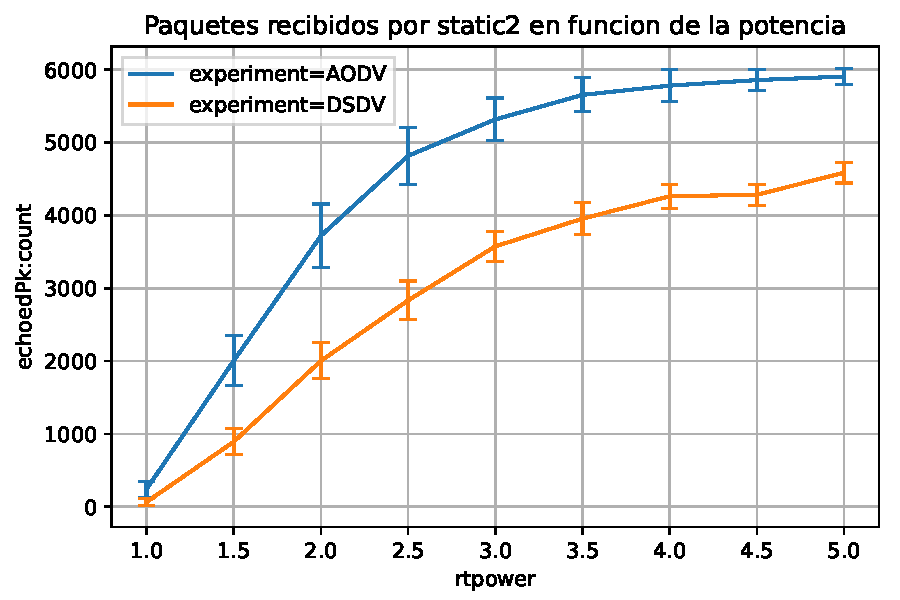
\includegraphics{imaxes/graficas/ejer4_1.pdf}
    \caption{Gráfica paquetes recibidos en static2 en función de la potencia}
    \label{fig:ejer4_1}
\end{figure}

El gráfico \ref{fig:ejer4_1} muestra que el nodo final static2 recibe más paquetes con AODV que con DSDV según aumenta la potencia de transmisión. Esto ocurre debido a las diferencias en la forma de enrutamiento de ambos protocolos.

AODV actúa de forma reactiva, de forma que establece rutas únicamente cuando se necesitan. A medida que aumenta la potencia de transmisión, se incrementa el rango de cobertura y el número de rutas alternativas (Es bastante improbable que se pierdan rutas, pero pueden existir nuevas rutas más óptimas). Sin embargo, AODV se queda con la ruta que conoce y sabe que funciona, a no ser que se produzca un error, lo cual no es habitual al aumentar la potencia.

Sin embargo, DSDV es un protocolo proactivo, por lo que mantiene una tabla de enrutamiento actualizada en todo momento, lo que introduce una mayor sobrecarga debido al intercambio constante de actualizaciones. Además, este mecanismo necesita que todos los nodos recompongan sus tablas de enrutamiento con mensajes hello después de un cambio de un error por cambios en la topología, lo que hace que se pierda tiempo en ese proceso en vez de seguir enviando paquetes según la red se vuelve más compleja.

\section{Ejercicio 4.2}

\subsection{Obtén una gráfica similar para el número de nodos. Explica lo observado.?}

\begin{figure}[H]
    \centering
    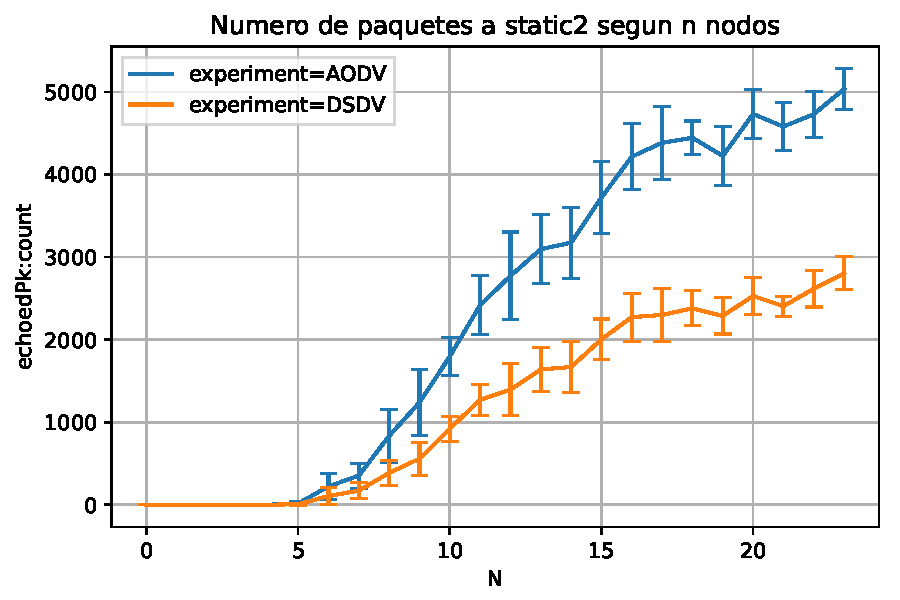
\includegraphics{imaxes/graficas/ejer4_2.pdf}
    \caption{Gráfica paquetes recibidos en static2 en función número de nodos}
    \label{fig:ejer4_2}
\end{figure}

Hay que destacar que en el .ini tenemos que llegue a 30 nodos pero por cuestiones de tiempo paramos en 23 ambos.

Como podemos ver en la gráfica \ref{fig:ejer4_2}, en AODV le llega a static2 mas paquetes que en DSDV. También hay que decir que en los dos aumenta pero AODV más rápido que en DSDV. La diferencia es:

En AODV en realidad no importa si aumenta el numero de nodos ya que una vez establece una ruta, a no ser que caiga, no va a dejar de usarla a no se que se rompa. 

En el caso de DSDV, le llega a static2 menos paquetes ya que al ir aumentando el número de nodos, los nodos vecinos ven que hay nuevos nodos por lo que van actualizando la tabla de enrutamiento entonces no se establece una ruta fija hasta que las tablas estean actualizadas.

También cabe destacar que por mucho que se aumente el número de nodos, va llegar un punto que para ambos protocolos el número de paquetes que le llega static2 va a ser constante.


\section{Ejercicio 4.3}

\subsection{Obtén una gráfica como las anteriores para la velocidad. Explica lo observado.}

\begin{figure}[H]
    \centering
    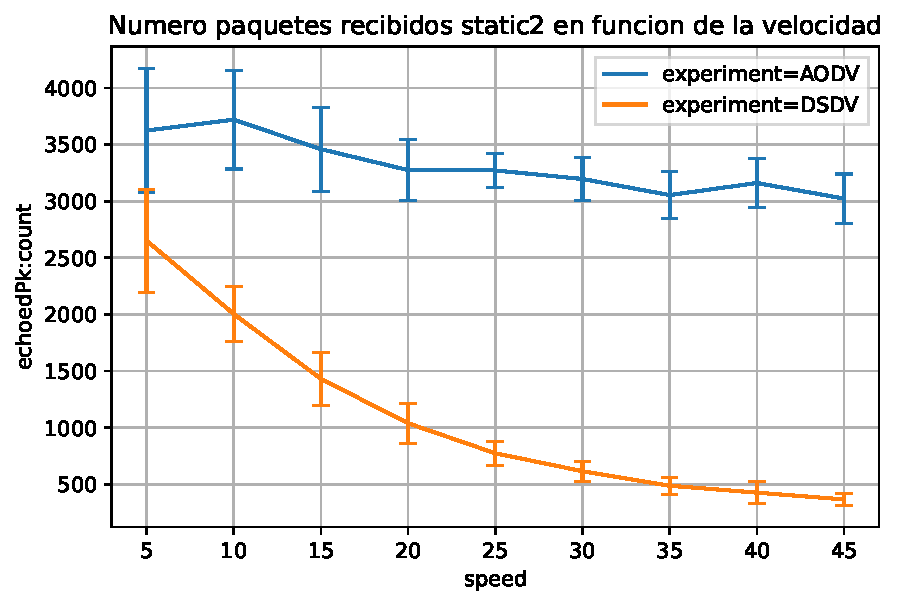
\includegraphics{imaxes/graficas/ejer4_3.pdf}
    \caption{Gráfica paquetes recibidos en static2 en función de la velocidad}
    \label{fig:ejer4_3}
\end{figure}

Como se puede ver en la gráfica \ref{fig:ejer4_3}, en AODV se mantiene más o menos el número de paquetes que le llega a static2, mientras que en DSDV a medida que la velocidad de los nodos aumenta, baja drásticamente los paquetes que le llegan a static2. Esto ocurre ya que en AODV, aunque los nodos se muevan mucho, esto no afecta a las rutas ya que aunque un nodo no sea alcanzable, si que lo es con otro por lo que siempre va haber una ruta y se va restablecer de forma rápida. En cambio en DSDV el movimientos continuo y aumento de velocidad hace que empeore la situación. Esto ocurre ya que en DSDV para que se establezca una ruta tienen que estar en todos los nodo, sus tablas de enrutamiento actualizadas, por lo que el movimiento continuo de los nodos dificulta la estabilización de las tablas por lo que no se establece una ruta y los paquetes no le llegan a static2. 

\section{Ejercicio 4.4}

\subsection{Para DSDV, obtén una gráfica del porcentaje de paquetes perdidos con diferentes valores de helloInterval.
Explica lo observado.}
